\section{Deterministyczne Automaty Skończone}
\subsection{Definicja}
\begin{definition}
    \textbf{Deterministyczny Automat Skończony} (DFA od deterministic finite automaton) to tupla:
    \[
        A = (Q, \Sigma, \delta, s, F)
    \]
    gdzie
    \begin{itemize}
        \item \( Q \) jest skończonym zbiorem stanów
        \item \( \Sigma \) jest skończonym alfabetem
        \item \( \delta: Q \times \Sigma \rightarrow Q \) jest funkcją przejścia
        \item \( s \in Q \) jest stanem startowym
        \item \( F \subseteq Q \) jest zbiorem stanów akceptujących (końcowych)
    \end{itemize}
\end{definition}

To jest bardzo abstrakcyjna i formalna definicja, w praktyce automat będziemy reprezentować jako graf skierowany, albo jako tabelkę przejść.

O automacie możemy myśleć jako o maszynie, która rozpoznaje czy zadane słowo należy do jakiegoś języka (związanego z tymże automatem). Zaczynamy w stanie startowym i przechodzimy do kolejnego stanu zjadając przy tym kolejne litery ze słowa.

Aby nieco sformalizować powyższe zdanie wprowadzamy funkcję \( \hat \delta \), która definiuje w jakim stanie kończymy jeśli zaczynamy w stanie \( q \) z danym słowem \( w \)
\begin{definition}
\( \hat \delta : Q \times \Sigma^* \rightarrow Q \)
\[
    \hat \delta(q, w) = \begin{cases}
    q & \text{ jeśli } w = \eps \\
    \delta(\hat \delta(q, x), a) & \text{ jeśli } w = xa, a \in \Sigma \\
    \end{cases}
\]
\end{definition}

\begin{definition}
    Językiem akceptowanym przez automat \( A = (Q, \Sigma, \delta, s, F) \) nazywamy
    \[
        L(A) = \set{w \in \Sigma^* \mid \hat \delta(s, w) \in F}
    \]
    
    Podobnie, słowo \( w \) jest akceptowane przez automat \( A \) jeśli \( w \in L(A) \)
\end{definition}


\subsection{Przykład}
Rozważmy automat zadany tabelą:
\begin{center}
    \begin{tabular}{c|c c}
        & \(a\) & \(b\) \\
        \hline
         \(q_0\) & \(q_1\) & \(q_0\) \\
         \(q_1\) & \(q_0\) & \(q_1\) \\
    \end{tabular}
\end{center}
\( s = q_0, F = \set{q_0} \)

\begin{figure}[H]
    \centering
    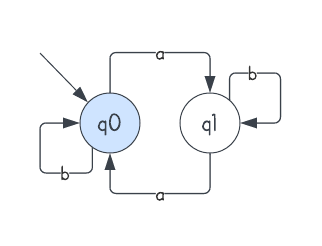
\includegraphics[scale=0.75]{img/even-a-automaton.png}
    \caption{Zadany automat w formie grafu}
\end{figure}


Niech \( L \) -- wszystkie słowa nad \( \set{a, b}^* \) w których występuje parzyście wiele \( a \).
Twierdzimy, że \( L(A) = L \).

\begin{proof} \( \)

\texttt{@PuchatyPompon}

\begin{description}
    \item ,,\(\subseteq\)''
    
    \item ,,\(\supseteq\)''
\end{description}
\end{proof}